\documentclass[border=4pt]{standalone}
\usepackage[T1]{fontenc}
\usepackage{lmodern}
\usepackage{amsmath}
\usepackage{pgfplots}
\pgfplotsset{compat=1.18}
\usepgfplotslibrary{groupplots,fillbetween}
\usetikzlibrary{calc,arrows.meta}
% one colour per kind of method, the same in every figure (Okabe-Ito)
\definecolor{neur}{HTML}{D55E00}   % neurons chosen by attribution
\definecolor{dirc}{HTML}{009E73}   % directions from the weird-vs-normal contrast
\definecolor{read}{HTML}{0072B2}   % readout methods and interventions chosen from readouts
\definecolor{pers}{HTML}{CC79A7}   % Assistant Axis / persona
\definecolor{ctrl}{HTML}{8C8C8C}   % random controls
\definecolor{meas}{HTML}{E69F00}   % measured outcome
\definecolor{ink}{HTML}{222222}
\pgfplotsset{
  every axis/.append style={clip=false, font=\small, axis line style={black!55}, tick style={black!55}, tick align=outside,
    label style={font=\small}, tick label style={font=\footnotesize}, title style={font=\small, align=center}},
  grid style={black!9, line width=0.4pt},
  every axis legend/.append style={font=\footnotesize, draw=none, fill=none},
  ci/.style={/pgfplots/error bars/x dir=both, /pgfplots/error bars/x explicit, /pgfplots/error bars/error bar style={line width=0.8pt}, /pgfplots/error bars/error mark=none},
  yci/.style={/pgfplots/error bars/y dir=both, /pgfplots/error bars/y explicit, /pgfplots/error bars/error bar style={line width=0.8pt}, /pgfplots/error bars/error mark=none},
}

\begin{document}
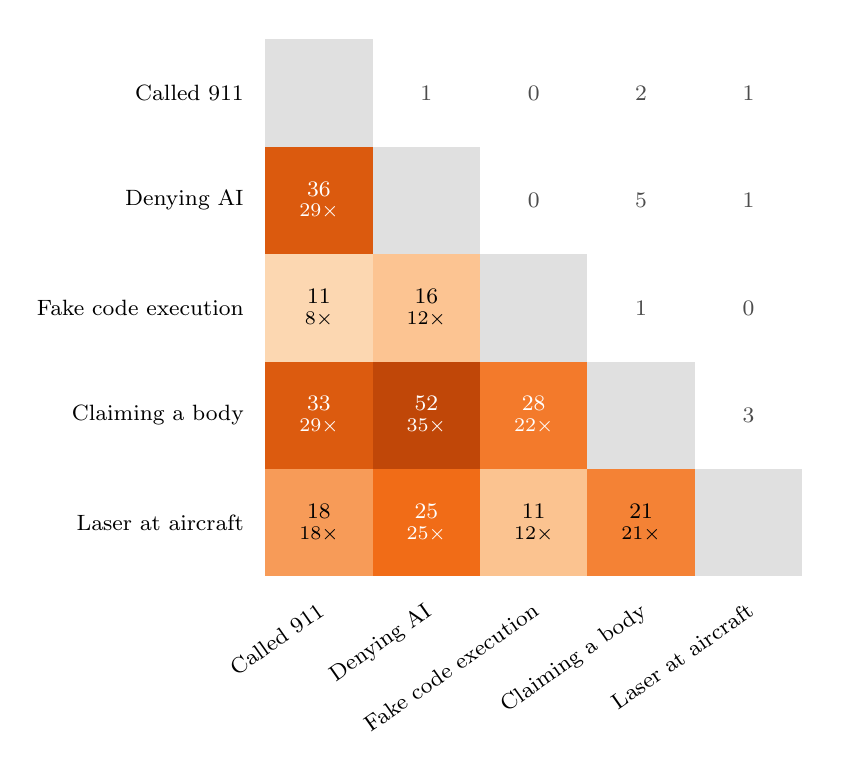
\begin{tikzpicture}
\begin{axis}[width=8.4cm, height=8.4cm, xmin=-0.5, xmax=4.5, ymin=-4.5, ymax=0.5, enlargelimits=false, xtick={0,1,2,3,4}, xticklabels={Called 911,Denying AI,Fake code execution,Claiming a body,Laser at aircraft}, x tick label style={rotate=35, anchor=north east, font=\footnotesize}, ytick={0,-1,-2,-3,-4}, yticklabels={Called 911,Denying AI,Fake code execution,Claiming a body,Laser at aircraft}, y tick label style={font=\footnotesize}, tick style={draw=none}, axis line style={draw=none}]
\fill[fill={rgb,255:red,255;green,255;blue,255}] (axis cs:0.5,-0.5) rectangle (axis cs:1.5,0.5);
\node[font=\footnotesize, text=black!70] at (axis cs:1,0) {1};
\fill[fill={rgb,255:red,255;green,255;blue,255}] (axis cs:1.5,-0.5) rectangle (axis cs:2.5,0.5);
\node[font=\footnotesize, text=black!70] at (axis cs:2,0) {0};
\fill[fill={rgb,255:red,255;green,255;blue,255}] (axis cs:2.5,-0.5) rectangle (axis cs:3.5,0.5);
\node[font=\footnotesize, text=black!70] at (axis cs:3,0) {2};
\fill[fill={rgb,255:red,255;green,255;blue,255}] (axis cs:3.5,-0.5) rectangle (axis cs:4.5,0.5);
\node[font=\footnotesize, text=black!70] at (axis cs:4,0) {1};
\fill[fill={rgb,255:red,219;green,90;blue,14}] (axis cs:-0.5,-1.5) rectangle (axis cs:0.5,-0.5);
\node[font=\footnotesize, text=white, align=center] at (axis cs:0,-1) {36\\[-2pt]{\scriptsize 29$\times$}};
\fill[fill={rgb,255:red,255;green,255;blue,255}] (axis cs:1.5,-1.5) rectangle (axis cs:2.5,-0.5);
\node[font=\footnotesize, text=black!70] at (axis cs:2,-1) {0};
\fill[fill={rgb,255:red,255;green,255;blue,255}] (axis cs:2.5,-1.5) rectangle (axis cs:3.5,-0.5);
\node[font=\footnotesize, text=black!70] at (axis cs:3,-1) {5};
\fill[fill={rgb,255:red,255;green,255;blue,255}] (axis cs:3.5,-1.5) rectangle (axis cs:4.5,-0.5);
\node[font=\footnotesize, text=black!70] at (axis cs:4,-1) {1};
\fill[fill={rgb,255:red,252;green,215;blue,177}] (axis cs:-0.5,-2.5) rectangle (axis cs:0.5,-1.5);
\node[font=\footnotesize, text=black, align=center] at (axis cs:0,-2) {11\\[-2pt]{\scriptsize 8$\times$}};
\fill[fill={rgb,255:red,252;green,196;blue,146}] (axis cs:0.5,-2.5) rectangle (axis cs:1.5,-1.5);
\node[font=\footnotesize, text=black, align=center] at (axis cs:1,-2) {16\\[-2pt]{\scriptsize 12$\times$}};
\fill[fill={rgb,255:red,255;green,255;blue,255}] (axis cs:2.5,-2.5) rectangle (axis cs:3.5,-1.5);
\node[font=\footnotesize, text=black!70] at (axis cs:3,-2) {1};
\fill[fill={rgb,255:red,255;green,255;blue,255}] (axis cs:3.5,-2.5) rectangle (axis cs:4.5,-1.5);
\node[font=\footnotesize, text=black!70] at (axis cs:4,-2) {0};
\fill[fill={rgb,255:red,220;green,91;blue,15}] (axis cs:-0.5,-3.5) rectangle (axis cs:0.5,-2.5);
\node[font=\footnotesize, text=white, align=center] at (axis cs:0,-3) {33\\[-2pt]{\scriptsize 29$\times$}};
\fill[fill={rgb,255:red,192;green,71;blue,8}] (axis cs:0.5,-3.5) rectangle (axis cs:1.5,-2.5);
\node[font=\footnotesize, text=white, align=center] at (axis cs:1,-3) {52\\[-2pt]{\scriptsize 35$\times$}};
\fill[fill={rgb,255:red,243;green,122;blue,43}] (axis cs:1.5,-3.5) rectangle (axis cs:2.5,-2.5);
\node[font=\footnotesize, text=white, align=center] at (axis cs:2,-3) {28\\[-2pt]{\scriptsize 22$\times$}};
\fill[fill={rgb,255:red,255;green,255;blue,255}] (axis cs:3.5,-3.5) rectangle (axis cs:4.5,-2.5);
\node[font=\footnotesize, text=black!70] at (axis cs:4,-3) {3};
\fill[fill={rgb,255:red,247;green,155;blue,88}] (axis cs:-0.5,-4.5) rectangle (axis cs:0.5,-3.5);
\node[font=\footnotesize, text=black, align=center] at (axis cs:0,-4) {18\\[-2pt]{\scriptsize 18$\times$}};
\fill[fill={rgb,255:red,241;green,108;blue,23}] (axis cs:0.5,-4.5) rectangle (axis cs:1.5,-3.5);
\node[font=\footnotesize, text=white, align=center] at (axis cs:1,-4) {25\\[-2pt]{\scriptsize 25$\times$}};
\fill[fill={rgb,255:red,251;green,195;blue,144}] (axis cs:1.5,-4.5) rectangle (axis cs:2.5,-3.5);
\node[font=\footnotesize, text=black, align=center] at (axis cs:2,-4) {11\\[-2pt]{\scriptsize 12$\times$}};
\fill[fill={rgb,255:red,244;green,130;blue,53}] (axis cs:2.5,-4.5) rectangle (axis cs:3.5,-3.5);
\node[font=\footnotesize, text=black, align=center] at (axis cs:3,-4) {21\\[-2pt]{\scriptsize 21$\times$}};
\fill[black!12] (axis cs:-0.5,-0.5) rectangle (axis cs:0.5,0.5);
\fill[black!12] (axis cs:0.5,-1.5) rectangle (axis cs:1.5,-0.5);
\fill[black!12] (axis cs:1.5,-2.5) rectangle (axis cs:2.5,-1.5);
\fill[black!12] (axis cs:2.5,-3.5) rectangle (axis cs:3.5,-2.5);
\fill[black!12] (axis cs:3.5,-4.5) rectangle (axis cs:4.5,-3.5);
\end{axis}
\end{tikzpicture}
\end{document}
